\subsection{Эмблематическая сущность логотипа}

В заключительном параграфе мы обратимся к определению границ семантического поля и социального
статуса логотипа. Номинально логотип, мы говорили ранее, есть общераспространенный знак-переменная
обозначения или маркировки объектов потребления и их производителей. В повседневном общении и в
специальной литературе он может называться товарным знаком, торговой маркой, маркой,
этикеткой-лейблом, символом, брендом и эмблемой.  Отсутствие единого представления о логотипе, с
одной стороны, отражает  субъективное желание пользователей и потребителей наделить знак удобными
или воображаемыми качествами, в целях использования в социально-экономической практике. С другой
стороны, с точки зрения практики лого дизайна, известная произвольность  использования термина
отражает  эклектичность его дизайна и принципов композиции, объективно вытекающих из необходимости
учитывать и удовлетворять желание заказчика. Как показывает опыт, отношение заказчика к выбору
своего логотипа сегодня носит отчетливо выраженный мифотворческий характер. Логотип в данном случае
представляется ему элементом  своего публичного образа или имиджа, тем, что А.Ф. Лосев называет
разрисовкой, картинным излучением личности \autocite[][94]{losev1991}. Для лояльного потребителя
однако логотип, по всей видимости, значим не столько своими мифотворческими потенциями, сколько
тотемической привлекательностью, способностью быть знаком клановой, родовой
принадлежности. Или иначе: знаком принадлежности некоему массовому сообществу. Терминологически
мифотворческие и тотемические возможности логотипа реализуются через его эмблематическую ипостась.
Мы уже рассуждали об исторической связи логотипа с геральдической эмблемой.  Теперь мы рассмотрим
эту аналогию более подробно.

\subsubsection{Границы эмблематического в логотипе}

Эмблематичность представлена в логотипе главным образом тремя свойствами. Во-первых, по внешней
форме исполнения -- сочетание изображения и слова -- логотип может композиционно напоминать
эмблему (рис.~\ref{fig:twins}). Даже в тех случаях, когда мы имеем дело с логотипами, состоящими из
одного вербального элемента или слова (рис.~\ref{fig:maroc}), форма исполнения данного элемента
носит отчетливо выраженный изобразительный характер. Слово-название в логотипе не пишется, а
изображается. Во-вторых, по своей внутренней мотивировке и первоочередному практическому назначению,
логотип, точно также как и эмблема, синхронически может иметь только один фиксированный смысл. В
данном случае: дифференциально обозначать и сигнализировать о присутствии и деятельности
компании-производителя на рынке товаров услуг и предполагаемом высоком качестве ее
продукции. В-третьих, по своему замыслу и основному символическому назначению логотип, подобно
эмблеме, является свернутым мнемоническим блоком, призванный транслировать во времени уникальный
ценностный статус компании-производителя и ее продукции, с одной стороны.  С другой стороны, внушать
целевому массовому потребителю ощущение эмоциональной сопричастности древней традиции, мистически
глубокому, но не до конца понятному смыслу, или, напротив, сопричастность новому технологическому
прорыву, модному тренду, революционному движению в будущее.  Иными словами, однозначность логотипа
во временном континууме предрасположена к энтропии, когда изначально жестко фиксированные внешние и
внутренние связи переформулируются, давая рождение новым смыслам.

\begin{figure}[h!]
  \centering
  
\includegraphics[width=.5\linewidth]{images/twins}
  \caption{Логотип <<Близнецы>>}
  \label{fig:twins}
\end{figure}

\begin{figure}[h!]
  \centering
  
\includegraphics[width=.5\linewidth]{images/maroc}
  \caption{Логотип <<Принц Марокко>>}
  \label{fig:maroc}
\end{figure}

Таким образом, логотип и эмблема нетождественны понятийно, и смысловое и формальное сходство между
ними носит лишь временный, этапный характер.  Развернем наши тезисы.

\paragraph{Эмблематическое сочетание}
Современная эмблема – это амальгам формы, образа и имени\hyp{}идентификатора. Она может представлять
собой простое замкнутое построение со стилизованной надписью или изысканно-витиеватым изображением
скрытых смыслов или мотивов. Как таковая эмблема сегодня обычно используются для идентификации
спортивных команд и престижных организаций или корпораций – предположительно, как мы отмечали,  по
аналогии с использованием фамильных гербов средневековой знатью. По своему замыслу современная
эмблема позволяет  массовому потребителю, -- каковым является, в том числе и спортивный болельщик
-- выстроить более тесную коммуникацию с брендом, особенно если она представляют команду или клуб.
С другой стороны, на утилитарном уровне, эмблема выразительно смотрится и на упаковке современных
товаров, как, например, эмблема одного из старейших брендов в Великобритании Lyle’s Golden
Syrup (рис.~\ref{fig:syrop}). С момента своего появления в 1904 году упаковка и логотип компании изменялись
лишь незначительно, придавая имиджу продукции компании значимый и хорошо продающийся ностальгический
статус старинной традиции.

\begin{figure}[h!]
  \centering
  
\includegraphics[width=.3\linewidth]{images/goldensyrop}
  \caption{Золотой сироп Лайлс}
  \label{fig:syrop}
\end{figure}

В современной эмблеме соположение вербального элемента и изображения\hyp{}рисунка далеко не всегда
самоочевидно, что само по себе имеет принципиальное значение. Изображение должно сообщать
потребителю нечто иное, не совпадающее и не дублирующее словесное обозначение-подпись. Объяснение
рисунка в эмблеме интерпретатором призвано одновременно как истолковать смысл изображаемого, так и
констатировать семантическую обусловленность изображения и слова. Иначе говоря, оба текста,
изначально представляющие собой разные языки, необходимо приравниваются друг к другу волевым
решением автора, с одной стороны, и интерпретирующим прочтением потребителя, с другой. Эмблема
представляет собой разновидность усиленного фразеологизма,  поскольку за элементами эмблемы
сохраняется право определенной автономии, равно как и возможность образования нового смысла при их
сопоставлении, не равного смыслу каждого из этих элементов в отдельности. Такое сочетание мы
называем эмблематическим. То есть, свободное сочетание некоторого стандартного набора иконических
и вербальных элементов, когда одно и то же изображение может сопровождаться различными подписями, и
одно одна и та же подпись может прилагаться к различным изображениям. Последнее, в частности,
объясняет острую проблему защиты авторского права в лого дизайне, где плагиат и визуальная кража
оригинальных дизайнерских решений носят массовый характер.

Далее, как вербальный, так иконический элементы в эмблеме по объему вмещаемых понятий могут занимать
по отношению друг к другу
\begin{enumerate*}[label=\asbuk*)]
\item обобщающую (свертывающую) позицию и
\item индивидуализирующую (развертывающую) позицию.
\end{enumerate*}
Или проще: по принципу <<свертывание-развертывание>>.  Иконический знак
ориентирован на обозначение единичного, конкретного объекта. Конвенциональный вербальный знак, по
причине своей абстрактности, стремится обозначить любой объект или даже все объекты.

Возникающее внутреннее противоречие оказывается чрезвычайно продуктивным.

Разная природа знаков, составляющих эмблему, позволяет эффективно разрешать его, поскольку в
эмблематическом сочетании значим не сколько логико-семантический объем каждого отдельного
сополагаемого понятия, сколько приведение того и другого к общему знаменателю. Более конкретному,
чем конвенциональный словесный знак, и более абстрактному, чем иконический знак. Если каждая
отдельная составляющая эмблемы может быть многозначной, то их сочетание дает однозначный смысл. По
аналогии с естественным языком, можно было бы сказать, что элементы, образующие эмблему, выполняют
смыслоразличительную функцию, в то время как эмблема в целом -- смыслообразующую. При этом эмблема,
возникающая как результат симметрически замкнутого процесса: от конкретного к абстрактному и снова к
конкретному, может означать только самое себя, т.е. знак с жесткой системой внутренней детерминации
составляющих элементов.

\paragraph{Мнемоническая функция эмблемы}

Из сказанного следует, что эмблема, выполняя свое задание в процессе взаимного указания элементов
друг на друга, оказывается исключительно важным знаком для исполнения ею функции мнемонической
стабилизации смысла. Эмблематический знак, будучи идеальным футляром для памяти, дает возможность
одновременно хранить информацию о некоторых абстрактных свойствах, составляющих ее означаемое, с
одной стороны, и информацию о конкретном объекте предметного мира, потенциально или реально им
соответствующих, с другой. Идея замкнутости, адекватности себе, сопротивляемости переменам, как мы
показали выше, составляет суть эмблемы и позволяет рассматривать ее в качестве механизма хранения
информации. Во всяком случае, еще древние руководства по мнемотехнике советовали запоминать
словесные тексты и абстрактные конструкции, сополагая их с яркими изображениями\autocite[][49]{grigoreva2005}.

Эмблематический по форме прием запоминания использовал, например, И. В. Гете: <<Интересный для него
предмет или местность он набрасывал на бумаге с помощью немногих штрихов, детали же он восполнял
словами, которые вписывал тут же на рисунке. Эти удивительные художественные гибриды позволяли ему в
точности восстанавливать в памяти любую местность (Localitat), которая могла понадобиться ему для
стихотворения или рассказа>>\autocite[][219]{bahtin1979}. Аналогичный
синтетический прием описывает А. Р. Лурия на примере человека, обладающего феноменальной памятью,
для которого наиболее простым способом запоминания словесного текста было последовательное
расположение слов в ряды знакомых с детства образов вдоль какой-нибудь дороги, домов, заборов,
витрин магазинов и т.д. в родном городе \autocite[]{luria1979}.
Примечательно, что механизм памяти срабатывал даже в том случае, когда не
существовало никакой очевидной семантической зависимости между словом и тем объектом, у которого оно
помещалось. Семантическая связь возникает как бы сама собой. Наконец, на основе жизненного опыта,
схожие приемы мнемотехники рекомендует и Д. Карнеги в своих популярных руководствах о том, как
добиться личного успеха в обществе \autocite[][237--420]{karnegi1996}.

Должно быть понятно, что запечатленная в эмблеме информация одновременно является смысловой
единицей. Точнее: единицей одного смысла, при этом непродолжительно действующей единицей.  Символу,
как мы говорили в конце первой главы, свойственно медленное накопление социокультурной памяти.  Его
новый смысл складывается из постепенных незаметных изменений в оттенках значения знака и неизбежно
возникающая при энтропия создает возможность полной трансформации его первоначального
смысла. Напротив, эмблематическое сочетание, по выражению И. Григорьевой, это <<информационный взрыв,
за которым следует полный штиль>> \autocite[][50]{grigoreva2005} В этом ее сильная и слабая стороны. Сильная
состоит в том, что превращает эмблему в готовый блок памяти, который при соответствующих условиях
внедрять в массовое сознание. Такой блок будет убеждать автоматически, практически не оставляя места
для сомнения в правильности предлагаемого высказывания. На этом принципе, как известно, базируется
рекламное сообщение, предполагающее максимально пассивное поглощение готовой информации.  Слабая
сторона выражается в том, что неизбежный распад эмблемы как единицы во времени, при котором
составляющие ее элементы получают возможность независимого функционирования, выводит ее из сферы
строгого эмблематического употребления в сферу стихийного и слабоуправляемого символического
смыслопорождения. Означаемое и означающее здесь зависят в первую очередь от позиции наблюдателя и,
следовательно, носят относительный характер. Логотип, рассматриваемый как часть маркетинговой
стратегии, разумеется, по целевому назначению ничем не отличается от готового мнемонического блока
эмблемы.

\paragraph{Рекламное воздействие коммерческой эмблемы}

Коммерческая эмблема, как и реклама в целом, соблазнительно предлагает массовому
потребителю заместить себя в воображении неким абстрактным, идеальным телом,
получающим наслаждение от вполне конкретных удовольствий. Или же наоборот:
получающим некие абстрактные удовольствия от конкретных товаров потребления.
Эмблемы рекламы по своему психологическому замыслу не должны замечаться сознанием.
Ожидается, что при максимальной пассивности мыслительных процессов в сознании
потребителя, информационный блок незаметно проникает в лимбический центр  мозга
и эффективно формирует перцептивный дубликат-заменитель его реального бытия в
реальном мире. Критичность восприятия блокирует суггестию, как отмечает, например,
М.К.~Рыклин, рассуждая о рекламных изображениях в московском метрополитене:
<<Характерная черта изображений в московском метро -- их незаметность для
протекающей мимо, как бы сквозь них, массы. И это несмотря на их очевидную,
бьющую в глаза фактурность. Превращение этих изображений в объект созерцания --
акт крайне агрессивный, нередко связанный для них с летальным
исходом>>\autocite[][41]{ryklin1992}.
Иначе говоря, рекламную коммерческую эмблему важно не замечать, но необходимо
добиться ее функционирования в качестве привычного естественного фона, как это
видно в следующем примере.

В 2010 году на восемьдесят второй церемонии вручения премии Академии
кинематографических искусств и наук в Лос-Анджелесе в категории <<Лучший
анимационный короткометражный фильм>> премию <<Оскар>> получил французский
мультфильм <<Логорама>> (Logorama). Годом раньше мультфильм получил в 2009 году
премию за <<Лучший короткометражный фильм>> на Стокгольмском кинофестивале и премию
Prix Kodak на кинофестивале в Каннах. Фильм показывает один день из жизни
города-прототипа Лос-Анджелеса, который помимо всего прочего знаменит еще и
тем, что в нем представлено огромное количество рекламы. Действительно, фильм
буквально кишит изображениями логотипов известных компаний, их слоганов и маскотов.
За 16 минут эфирного времени в поле зрения зрителей попадают упоминания примерно
о 2500 компаниях. Здесь практически все является логотипами брендов -- люди,
дома, техника. Имена героев говорят сами за себя: Playboy-кролики,
Linux-пингвины, MGM-львы в зоопарке, Michelin-полицейские выслеживают
преступника по имени Рональд МакДональд, и т.д. В финале мультфильма-боевика
<<Логорама>> клоун-террорист Рональд Макдональд разрушает эмблематичный мир
красивых картинок. Мы видим, что планета, на которой происходят события,
вращается вокруг гигантского логотипа Пепси, а тот в свою очередь висит где-то
на краю логотипа Милки Уэй. Life is better than Milky Way.

В реальной жизни функцию клоуна-террориста, как наглядно продемонстрировали
французские кинематографисты, выполняет критическая рефлексия. Рефлексия убивает
коммерческую эмблему, показывает абсурдность ее претензий, разоблачает
иллюзорность благих намерений и исполнения несбыточных мечтаний. Коммерческая
эмблема, или более узко -- логотип, используемый уже не в качестве знака
маркировки, а в качестве рекламного приема, становится технологией манипуляции
восприятием потребителей, искажения реальности, или попросту --
технологией обмана. Нужно признать, тем не менее, что взятая сама по себе
коммерческая эмблема обманывает ничуть не больше любого другого знака, который
по определению не является тем, на что он указывает.

С другой стороны, как мы неоднократно подчеркивали, свое настоящее значение
знак получает лишь в социальной практике коммуникации, внутри конкретной
сферы его применения. В данном случае такой сферой является реклама. Фабуляция,
гипертрофированное преувеличение и иллюзия имманентны технологии рекламы. Можно
сказать, они являются ее modus vivendi. Современная реклама, превратившись в
повествовательную стратегию, предлагает потребителю уже не столько сам товар,
сколько его идею, имидж, комплекс положительных переживаний (experience),
которые не нуждаются в верификации. Любая произвольно-привлекательная аргументация
может с легкостью рекламировать любой товар. Любой сюжет, миф или ценностная
категория становятся строительным материалом для создания рекламного нарратива
и как таковые отбираются  по принципу эффективного воздействия на целевую
потребительскую массу. Соответственно, рекламный нарратив может быть виртуозным
и изобретательным в использовании приемов ассоциативного творческого
конструирования. В то же время, должно быть понятно, что разнообразие
используемых технических приемов совсем не обязательно предполагает разнообразие
используемых средств и методов. Как раз наоборот: методологически реклама
предсказуема и единообразна, поскольку функционально она соподчинена другой
мощной знаково-символической системе. Эта система называется деньги.

Деньги -- всеобщее меновое средство, безразличное к любым численно не
измеряемым ценностям. Подобно тому, как художник вкладывает все свое мастерство
в написание картины, чтобы превратить ее в деньги, в вещь, ничего общего с
живописью не имеющую, так и копирайтер и лого дизайнер вкладывают свое
мастерство в создание рекламного  нарратива, чтобы превратить его в деньги,
в вещь, ничего общего не имеющую ни с его  содержанием, ни с его художественной
формой. Самый простой вид рекламного продукта и рекламного воздействия
рассчитаны на однократную выгоду, обычно в тех случаях, когда речь идет о
коммерческой рекламе материальных товаров.  Совсем иначе выглядят те
многочисленные случаи, когда рекламные технологии и механизмы переносятся из
сферы сбыта товаров и услуг в социальную жизнь общества с целью формирования
новых потребностей и долгосрочных поведенческих стратегий потребителей.

Речь здесь идет, во-первых, о создании масс лояльных потребителей, объединенных
некоей общей положительной эмоцией, заставляющих их  пользоваться услугами
конкретного продавца, компании производителя или фирмы, независимо от наличия
других, более выгодных предложений. Современного потребителя уже трудно назвать
просто покупателем. Он занимается шоппингом. Между шоппингом и походом в магазин
за покупками есть одно существенное различие. Последнее ориентировано на
приобретение необходимых товаров, удовлетворение материальных потребностей. В
то время как шоппинг – это разновидность социального общения, форма
увлекательного времяпрепровождения вне дома, обычно в торговых центрах, в
компании друзей или членов семьи. Покупка конкретного товара здесь вторична.
Факт покупки не столь значим, как эмоциональный социальный контакт в
сакрализованном пространстве торгового центра, насыщенном образами товаров и
услуг, потребного будущего, равно как и комфортными образцами для
самоидентификации и сравнения. Психологически, иллюзия лучшего будущего,
создаваемая современной рекламной технологией, по-видимому, сходна с иллюзией,
возникающей при прочтении увлекательного романа или просмотра захватывающего
фильма. И в том и в другом случае мы имеем дело с технологией удовольствия и
радости, когерентно произвольной <<пластической силой>>, по определению
А.Н.~Веселовского, способной творить безотносительно к теме, идее или сюжету
предлагаемого нарратива. Логотип как инструмент такой технологии является
эмблематическим фиксатором,  инвариантной точкой, вокруг которой выстраивается
рекламный нарратив. Но, как и любое эмблематическое сочетание, логотип и
реклама утрачивают свою эмблематическую значимость, оказавшись в фокусе
рефлексирующего сознания.

Два уровня рефлексии разрушают эмблематическую конструкцию: что изображается и
как это проверить? Вместе с тем, рефлексирующее сознание по определению не
может быть массовым. Поэтому эмблематические сочетания, к каковым относится
и логотип, успешно выполняют свою мнемоническую функцию анкера в массовом
сознании потребителей, позволяющим эффективно формировать и управлять
потребительскими массами.

Прежде чем перейти к  суггестивным механизмам воздействия, обобщим сказанное.
\begin{enumerate}
\item Логотип подобен эмблематическому сочетанию по структурной сочетаемости
  изобразительных и вербальных элементов, образующих бинарную оппозицию,
  один из членов которой -- образ, изображение -- более предпочтителен, чем второй.
\item В коммуникативном плане, целесообразно различать две ипостаси логотипа:
  \begin{enumerate*}[label=\asbuk*)]
  \item логотип как маркировочный знак идентификации и
  \item логотип как инструмент-технология создания привлекательного имиджа
    производителя, с одной стороны, и имиджа лояльного потребителя, с другой.
  \end{enumerate*}
  Во второй ипостаси логотип становится эмблематическим агентом рекламной
  коммуникации.
\item Подобно эмблеме логотип выполняет мнемоническую функцию в том смысле,
  что представляет собой  готовый блок памяти, внедряемый в массовое сознание
  потребителей. Такой блок становится анкером потребительской активности и
  инструментом формирования массовых сообществ.
\item Эмблематичность логотипа как коммерческого знака носит временный
  характер, поскольку подвержена энтропии, распаду фиксированного смысла под
  воздействием внешних факторов, таких как, например, склонность массовых
  потребителей к инклюзивному смыслопорождению. Иначе говоря, граница между
  логотипом-эмблемой и логотипом-символом условна и прозрачна.
\end{enumerate}

\subsubsection{Суггестивные механизмы логотипа-эмблемы}

В общем виде мы уже затрагивали вопрос о воздействии (суггестии) в первой главе
в связи с механизмами массообразования. Ниже мы конкретизируем нашу позицию
на материале лого дизайна.

\paragraph{Рекламное воздействие и  проблема внимания}

Воздействие-внушение может быть многоликим и разнообразным. Не будет большим
преувеличением сказать, что в той или иной форме с внушением мы сталкиваемся
повседневно и сами пользуемся им осознанно или неосознанно при выполнении
профессиональных обязанностей, в повседневно общении в семье, на отдыхе, в
кругу друзей и т.д. Наши предпочтения и вкусы зачастую являются результатом
чьих-то влияний, внушений или просто собственного самовнушения. Внушение
заложено в саму природу речевой деятельности и по этой причине распространено
повсеместно и сопровождает нас повсюду. В рекламе воздействие-внушение становится
специально организованным видом односторонней коммуникации, когда восприятие
коммерческой информации не встречает критических барьеров. В то же время,
рекламное внушение -- именно под эти углом зрения мы представляем сейчас
логотип -- принято выделять в особую манипуляторную деятельность, наделяя ее
при этом агрессивными, беспринципными качествами, наносящими непоправимый ущерб
человеческой психике. На самом деле группа рекламозависимых лиц, подверженных
прямому рекламному воздействию, сравнительно немногочисленная. В нее входят
дети, подростки, пожилые люди и больные слабоумием. Взрослый потребитель
воспринимает рекламу критично и осмысленно\autocite{roblesconsumer}.

Идеальная формула рекламного воздействия, сформулированная Дж.В.~Лундом в
1947~году -- AIDA (внимание, интерес, желание, действие), показывает
последовательные шаги воздействия на потенциального потребителя. Соответственно
оформляются и задачи такого воздействия: привлечь внимание, вызвать интерес,
способствовать появлению желания приобрести товар, спровоцировать конкретные
действия\autocite{lund1947newspaper}. Реальная жизнь, тем не менее, очень быстро
показала несостоятельность такой схемы. Выяснилось, в частности, что реклама
не только может привлекать внимание потребителей, но также может вызывать и
внутренний протест, равно как и желание приобрести товар совсем не обязательно
приводит к его покупке.

Первая серьезная проблема, с которой сталкивается любой изготовитель рекламы,
это избирательность нашего восприятия. Наш мозг автоматически фильтрует поток
получаемых ощущений, видоизменяя их, отбирая те, которые соотносятся с
предыдущим опытом, с нашими убеждениями, потребностями, желаниями и мнениями.
Мы можем сосредотачивать свое внимание на одних вещах и игнорировать другие.
Скажем, в одном периодическом издании могут быть размещены десятки  рекламных
сообщений, но средний потребитель позднее вспоминает лишь некоторые, в то время
как собственно влияние на него оказывают единицы. Парадокс рекламной
деятельности состоит в том, что рекламодатель, затрачивая миллионные суммы на
свою рекламу в национальных СМИ, на рекламные компании, дизайн упаковки и
оформление товарных витрин, нередко может при последующем опросе оказаться
перед фактом, что мало кто из потребителей помнит что-либо о его товаре и
проведенных рекламных мероприятиях. Более того, некоторые потребители не помнят
ничего. Растущее, как снежный ком, количество моделей и серий товаров и услуг,
казалось бы,  полностью обесценивает усилия копирайтеров и дизайнеров по поиску
уникальных сторон товаров и марок, равно как и  по конструированию незабываемых
ассоциативных комплексов памяти. Во всяком случае, изменение концепции
рекламного образа становится насущной проблемой.

\paragraph{Суггестивные предпосылки рекламного образа}
Традиционное представление о рекламном образе предполагает достоверную
корреляцию между изображением и изображаемым предметом. Но при массовом
производстве похожих товаров становится понятно, что достоверность не может
быть образной, а образность совсем не обязательно должна отражать настоящее
положение дел. В результате, эмблематический по сути рекламный образ отдалился
от рекламируемого предмета, став  одновременно более абстрактным и более
независимым. При этом образность и психологическая дифференциация вышли на
первый план, в то время как качество и убедительность заняли подчинительное
положение. Такое смещение акцентов в рекламной деятельности неожиданно получило
широкий резонанс в гуманитарных науках, в которых -- в крайнем теоретическом
пределе -- современной рекламе приписывается статус идеологической инстанции,
призванной <<оправдывать>> потребление, иррационально воздействовать на умы
граждан и служить апологетом капиталистического общественного устройства.
Согласно этому представлению, в массовом сознании рекламные образы образуют
единое целое и потребляются, ни больше, ни меньше, как фальсифицированная
картина мира, а обладание рекламными вещами создает у массового потребителя
ложное ощущение непосредственной связи с реальностью\autocite[][190-191]{bodriyar1999sistema}.
Несоответствие данного теоретического построения фактам повседневной жизни мы
уже отмечали,  поэтому обратимся непосредственно к техническим механизмам
воздействия в логотипе с точки зрения рекламного сообщения.

\paragraph{Суггестивность эмблематического рекламного сообщения}
Универсальное рекламное сообщение, как мы говорили раньше, носит эмблематический
характер. Если  до этого мы говорили в общем виде о двух составляющих --
изображении и подписи-имени, то теперь введем еще один смыслоразличительный
элемент -- цвет. Все вместе они образуют некую смысловую триаду. Цвет,
по-видимому, является самой простой составляющей. Вполне достаточно знать
закономерности воздействия цвета на психику, чтобы умело им пользоваться.
Можно различать три вида воздействия цвета: физическое, оптическое и
эмоциональное\autocite{tsoygner1971}\autocite{serov1997estetika}\autocite{kandinsky2001dohovnom}.

\emph{Физическое воздействие}. В данном случае речь идет о воздействии на
  физиологию человека. Сила воздействия зависит от количества цвета,
  его качества, времени воздействия, особенностей нервной системы, пола,
  возраста и прочих факторов. Из обычной палитры известно, например, что
  красный цвет возбуждает нервную систему, вызывает учащение дыхания и
  пульса. Синий цвет, напротив, оказывает тормозящее действие на нервную
  систему. Группа красного, желтого, оранжевого цветов являются цветами
  экстраверсии, т.е. импульса, обращенного наружу. Синий, фиолетовый,
  зеленый, с другой стороны,  интровертивные стимулируют импульсы, обращенные
  внутрь.

  Действие цвета совсем необязательно всегда ассоциативно. Точнее говорить о
  синестезии, т.е. о возбуждение одного органа чувств во время раздражения
  другого. В результате, цвета получают свою особую смысловую интерпретацию.
  Например, желто-коричневый может казаться сухим,  розовый -- слащавым,
  красный -- теплым, оранжевый -- кричащим, фиолетовый -- тяжелым, желтый -- легким.

\emph{Оптическое воздействие}. К этому виду воздействия следует отнести
  оптические явления или иллюзии, вызываемые цветом и изменяющие внешний вид
  предметов. Скажем, светлые цвета, такие как белый или желтый создают эффект
  иррадации. Они как бы распространяются на расположенные рядом с ними более
  темные цвета и уменьшают поверхности, окрашенные в эти цвета. Иррадиация, в частности, играет важную
  роль при конструировании шрифтов. Например, если буквы F и E сохраняют свою полную высоту, то высота
  таких букв как O и G, несколько уменьшаются. В то же время, еще больше уменьшаются буквы A и V из-за
  своих острых окончаний. Эти буквы кажутся ниже общей высоты строки.  Поэтому, чтобы они казались
  одинаковой высоты с остальными буквами строки, их уже при разметке следует вынести несколько вниз
  или вверх за приделы строки.

\begin{figure}[h!]
  \centering
  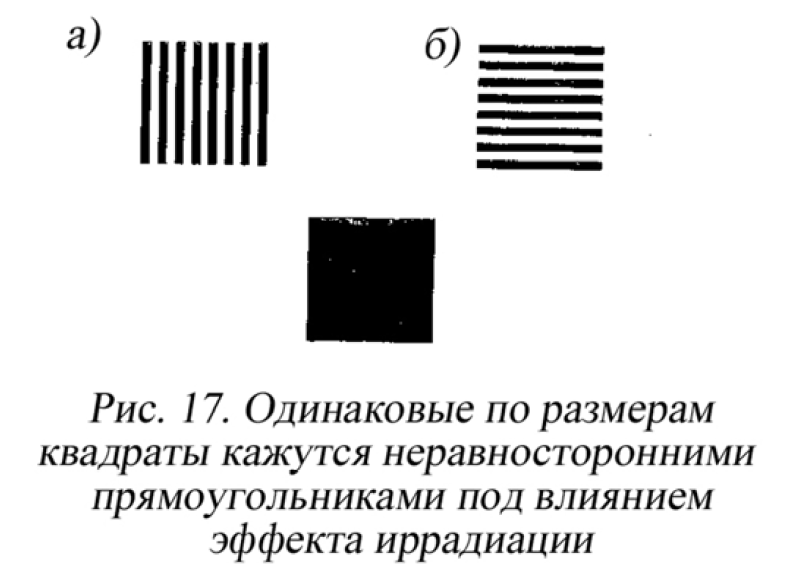
\includegraphics[width=.5\linewidth]{images/irradation}
  \caption{Эффект иррадации}
  \label{fig:irradation}
\end{figure}

  Наконец, эффектом иррадации объясняется и различное впечатление от
  поверхностей, с нанесенными на них продольными или поперечными полосками.
  Поле на рисунке слева (рис.~\ref{fig:irradation}) может казаться более низким, по сравнению с полем на рисунке справа, так как белый
  цвет, окружающий поля проникает между полосками наверху и внизу и визуально уменьшает высоту
  поля. Более обобщенно: желтый цвет зрительно как бы приподнимает
  поверхность, и она может казаться более обширной из-за эффекта иррадации. Если красный цвет
  приближается к нам, то голубой, напротив, удаляется. В то же время как плоскости, окрашенные в
  черный, фиолетовый или темно-синий цвета, зрительно уменьшаются и устремляются к низу.

\emph{Эмоциональное воздействие}. Этот вид воздействия тесно связан с
  оптическими свойствами цвета и говорит о переживаниях и чувствах, которые
  мы можем испытывать под влиянием того или иного цвета. Так, самый спокойный
  цвет -- зеленый. В нем нет движения и никаких признаков ни радости, ни грусти.
  Как таковой он благотворно действует на утомленных людей. Зеленый цвет
  становится более активным и оживленным, если в него ввести желтый. При
  добавлении синего, он, наоборот, делается более серьезным и вдумчивым и т.д.
  Выбор любимого цвета человеком определяется его характером и зависит, помимо
  всего прочего от социальных факторов. Более того характер и выразительность
  цвета может существенно меняться в зависимости от спектра личных ассоциаций.
  Ведь нередко мы пытается объяснить эмоциональное содержание того или иного
  цвета характером предметов, на которых мы обычно воспринимаем этот цвет.
  По этой причине устанавливать здесь какие-либо однозначные правила
  представляется нецелесообразным. Тем не менее, с некоторой вероятностью
  можно предположить, что красный цвет ассоциируется с огнем и страстью,
  желтый -- с солнцем, синий -- с небом или водой, зеленый -- с лесным массивом
  или лугами.

Таким образом, овладев языком цвета, можно выразить и протестный молодежный
максимализм, и подчеркнутый консерватизм, можно сделать образ вульгарным или
нежным, мужественным или женственным и т.д. Изображение и цвет взятые сами по
себе, будучи производными художественного творчества, в рекламном образе
сохраняют известную автономию. Законченный фиксированный смысл по эмблематическому
принципу ему придает подпись-имя или слоган. Внутри эмблематического сочетания
рекламного образа цвет и изображение сужают свой изначальный смысл до намека и
обрамляются вербальным текстом. Важно, что текст не истолковывает точно ни
изобразительные составляющие внутри эмблемы, ни сам рекламируемый предмет.
Вместо этого, триединое сочетание оформляется в виде некой легкой аллюзии, хотя
и по принципу жесткого внутреннего соподчинения, необходимого и достаточного,
как мы говорили, для массового воздействия. Рекламный образ в силу своей
иррациональности и высокой абстрактности означаемого тем не менее эффектно
указывает на некое пусть смутное, но искомое желаемое, с одной стороны, и
создает это желаемое, предлагая в него поверить, с другой.

\paragraph{Суггестивность образа компании в  графической эмблеме}

Образ компании, который несет ее название и графическая эмблема, включает в
себя несколько уровней.

Во-первых, это уровень содержательных ассоциаций. Скажем, название обычно
позволяет строить предположения о профиле компании, даже тогда, когда само
слово-название ничего не значит. Эмблемы, как и названия, могут различаться по
тому, направляют ли они ассоциации в том или ином направлении или вообще не
дают им никакой направленности. Конкретно-изобразительные элементы эмблем,
багет в форме буквы F в логотипе <<French Bakery>> или вешалки в форме куполов
индийского храма в логотипе <<My Indian Closet>>, являются основными носителями
образной информации этого уровня (рис.~\ref{fig:indiancloset}).

\begin{figure}[h!]
  \centering
  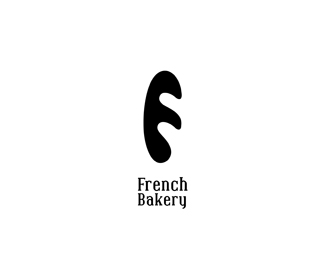
\includegraphics[width=.5\linewidth]{images/frenchb}
  \caption{Логотип <<Французская пекарня>>}
  \label{fig:indiancloset}
\end{figure}

\begin{figure}[h!]
  \centering
  
\includegraphics[width=.5\linewidth]{images/indiancloset}
  \caption{Логотип <<Мой индийский клозет>>}
  \label{fig:indiancloset}
\end{figure}

Во-вторых, это уровень культурных ассоциаций, по которым можно предполагать
национальную принадлежность и возможно  исторические корни компании. Определенные
ассоциации такого рода могут вызывать не только значащие
названия (<<Чухлома Лес>>, <<Застава>>, <<Пивград>>, <<Серебряная ладья>>), но
и бессмысленные (<<Альфа-Билд>>, <<Modeform>>, <<Воталиф>>, <<Авикос>>).
В эмблеме -- это изобразительные знаки и символы, содержащие в свернутом виде
заряженный эмоциональный опыт и способные непроизвольно воскрешать этот опыт
в подсознании. Это может быть чистая эмоция (Apple), равно как и символ с
общекультурным смыслом (Уроборос). Носителем культурных ассоциаций могут
выступать стилевые элементы или матричные графические фигуры. К последним
относятся, например, круг, крест, свастика, треугольник, закон 10:10,
равно как и базовый <<словарь>>, в который входят тотемные животные, череп,
глаза-окна-зеркала-двери-лестницы-пороги, уши-раковины-трубы-птицы
и~т.д\autocite{link:grigorevalj}.

В-третьих, это эмоциональная окраска звучания названия и изобразительных
элементов эмблемы. При использовании в названии искусственных или иностранных
слов, аббревиатур или акронимов по принципу семантического дифференциала именно
эта сторона выходит вперед. Качества, с которыми звуки подсознательно связываются
в нашем восприятии, могут быть быстрыми и медленными, холодными или горячими,
светлыми и темными, мягкими и жесткими
и~т.д\autocite{juravlev1991zvuk}. В зависимости от преобладания в слове-названии
звуков с той или иной эмоциональной окраской слово в целом тоже приобретает эту
окраску. Графически, точно так же как и звуки, ту или иную эмоциональную
нагрузку несут линии, цвета и другие изобразительные приемы, позволяющие
сделать ощущение знака в восприятии динамичным или устойчивым, легким или
тяжелым, мужественным или женственным и т.д. В то же время, первоначальная цель
графической эмблемы на первом этапе -- не глубокие чувства и переживания, а
фиксация взгляда, ясное и четкое восприятие. По этой причине знак должен быть
одновременно сложным и лаконичным, что достигается обычно через жесткую форму
конструктивного построения, преднамеренную искусственность и четкую геометрию.

Таким образом, в конструировании привлекательного ассоциативного образа компании
широко применяется суггестивная связь используемых выразительных средств с теми
или иными эмоциональными проявлениями. Так, прямые линии  могут выражать одно
состояние, ломаные -- другое, а кривые -- третье. Движение слева направо или
наоборот,  цвета, графические изобразительные формы и звуки речи -- все они
несут в себе те или иные относительно устойчивые эмоциональные значения,
незаметно воздействующие на восприятие массового потребителя, его
эмоционально-чувственную сферу, отвечая его потребностям, желаниям и ожиданиям,
которые по определению являются коллективными. Или иначе: входят в фонд
коллективного бессознательного.

\paragraph{Суггестивнось типического в логотипе}
Концептуально, типическое в логотипе обладает суггестивностью. Суггестивно,
например, повсеместное использование и воспроизведение логотипа на
многочисленных носителях. Подобно тому, как стилистический повтор в риторическом
высказывании рассчитан на оказание воздействия, фиксирует внимание
читателя (слушателя) на той или иной смысловой доминанте, так и логотип,
просто в силу своей повсеместности, своим присутствием непроизвольно
воздействует на потребителя, подчеркивая значимость и значительность
рекламируемого товара и его производителя. Назовем это внешним, эксплицитным
планом суггестии типического. Внутренним, имплицитным планом будет, с одной
стороны, аффектация, т.е. воздействие рекламного образа, вызывающее
кратковременные бурные эмоции. Аффектацию может стимулировать использование
приемов иронии, пародирования, деканонизация общеизвестных эстетических
ценностей. С другой стороны, внутренний план суггестии оформляет  использование
универсальных символов и стоящих за ними природных визуальных паттернов.
Дизайн логотипов в данном случае становится технологией коммуникации через
интуитивное чувство паттерна. Укорененность в природе обеспечивает ему
эстетичность, эффективность и долгосрочность воздействия\autocite[][9]{macnab2008decoding}. Остановимся
на этом подробнее.

К универсальным визуальным паттернам принято относить  круги, свастику, спирали,
разветвления, переплетения и изгибы, треугольники, квадраты и другие многоугольные
фигуры, и числа (1-9). Распознавание паттерна происходит через символ, визуальную
метафору, связанную с природной энергией, которую он выражают. Независимо от
конкретного языка, культуры или исторического периода, такой символ представляет
собой архетип чувства, с которым может идентифицироваться каждый, тем самым
поддерживая связь между глубинным природно-культурным опытом человечества и
современной повседневностью. По этой причине опознавание универсальных символов
и визуальных не вызывает особых трудностей. Проиллюстрируем сказанное на примере
круга, креста, свастики и спирали.
\begin{enumerate}
\item Круг. Круги присутствует во многих известных логотипах: NASA, Pepsi,
  AT\&T, Vodafone, Nissan, Volkswagen, BMW и~т.д. В одних случаях окружность
  просто очерчивает контур вокруг слова или графического элемента, работая
  как магический символ, ограждающий от злых сил и хранящий в себе благотворное
  влияние, в других он является формообразующим элементом.

\begin{figure}[h!]
  \centering
  
\includegraphics[width=.3\linewidth]{images/obamademo}
  \caption{Логотип Обамы и Демократической партии США}
  \label{fig:obamademo}
\end{figure}

   Так, например, новый
  логотип американской демократической партии, представленных в рамках нового
  визуального стиля с осени 2010~г. отошёл от традиционного изображения осла,
  раскрашенного в национальные цвета, и стал одной буквой D в круге, а точнее
  в букве O (рис.~\ref{fig:democrats}). Включенность в круг роднит новый логотип с логотипом
  избирательной компании президента США Б.~Обамы (2008). Логотип Обамы (рис.~\ref{fig:obama})
  изображает восходящее над горизонтом солнце нового дня. Образ солнца архетипичен
  и повсеместен в лого дизайне. Такая популярность, вероятно, говорит о том,
  что человечек до сих пор бессознательно сохраняет некоторые следы древнего
  преклонения перед солнцем и реализует эту потребность в современной
  коммерческой символике. Как бы то ни было, логотип-эмблема Обамы и буква О
  положили начало новому тренду в корпоративной айдентике 2011 года.
  Во время новой предвыборной компании на сайте демократов был размещен
  баннер с цифрами 2012, логотипом Обамы в 0 и вопросом <<Are you in?>>,
  что визуально можно перевести <<ты в круге?>> Безусловно, успех логотипа
  Обамы -- это не успех одного только знака. Символом, здесь, скорее,
  является обаятельная, харизматичная личность президента, нежели его
  эмблематический знак. Он -- отражение изменений, произошедших в политическом
  сознании американцев. Значения, которые продуцирует знак, только подкрепляют
  эту идею. В этой связи Обама -- это успешный бренд, который, как и любой
  коммерческий бренд, включает знак, имя бренда, репутацию, атмосферу,
  выстроившуюся вокруг него. Хороший логотип может иметь ценность сам по себе,
  и эта ценность только добавляет к ценности компании, товара или услуги.

\item Крест. Крест -- один из самых успешных универсальных символов, который
  когда-либо существовал. Он мгновенно узнаётся и  имеет большую силу
  воздействия. Первоначально, крест -- символ угнетения и страдания. Крест так
  же являлся атрибутом королевской власти и являлся важной частью
  геральдической символики. А учитывая различные культурные контексты,
  символы Красного Креста, Красного Полумесяца и Красного Кристалла
  используются в различных частях мира, чтобы представлять, что известно в
  Соединенных Штатах как Красный Крест.

\begin{figure}[h!]
  \centering
  \begin{subfigure}{.45\textwidth}
    \centering
    
\includegraphics[width=\linewidth]{images/cross1}
    \caption{Религиозный бренд <<Великий Я>>, Руди Хуртадо}

    \label{fig:cross3}
  \end{subfigure}
  \hfill
  \centering
  \begin{subfigure}{.45\textwidth}
    \centering
    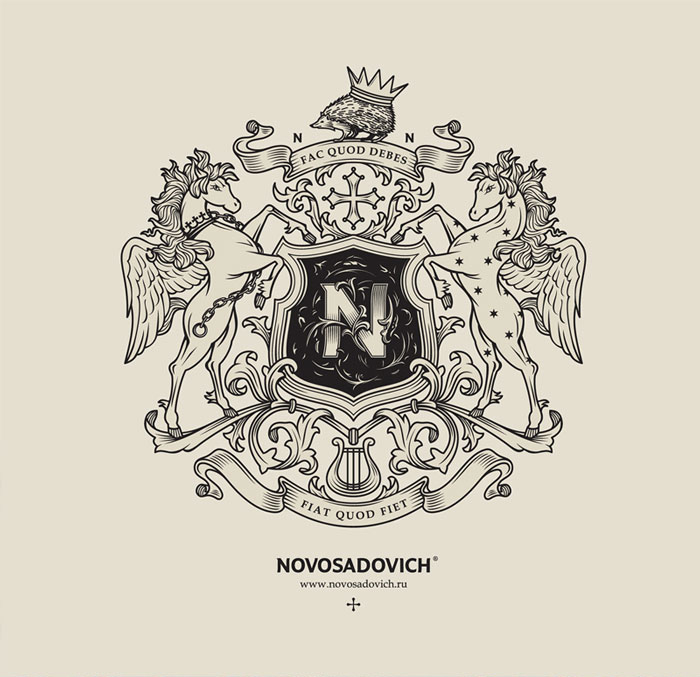
\includegraphics[width=\linewidth]{images/cross2}
    \caption{Герб для Надежды Новосадович, Денис Башев}

    \label{fig:cross2}
  \end{subfigure}
  \end{figure}

  Использование креста, по своей сути,
  осознается лого дизайнерами, как серьёзный символ и используется
  преимущественно только по прямому назначению, для логотипов религиозного
  характера, или в коммерческой геральдике (рис.~\ref{fig:cross1}, рис.~\ref{fig:cross2}).


\item Свастика. Мы уже упоминали о том, что свастика утратила своё исконное
  значение быть символом жизни, света и благополучия после того, как она была
  тиражирована немецкой дизайн студией <<Вильгельмверк>> и позднее отложилась в
  массовом сознании в качестве эмблемы германского фашизма. До этого свастику
  использовали в качестве символа удачи и счастливой жизни, на предметах быта,
  одежде, гербах и знамёнах, при оформлении храмов и домов, в коммерческих,
  рекламных и пропагандистских целях. Например, в 1925 <<Кока-кола>> выпустила
  <<счастливый брелок>> для карманных часов в форме свастики (рис.~\ref{fig:cocaswastica}).

  \begin{figure}[h!]
  \centering
  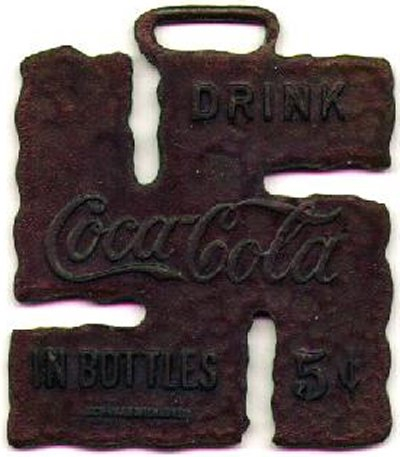
\includegraphics[width=.2\linewidth]{images/cocaswastica}
  \caption{Брелок для карманных часов <<Кока-кола>>, 1925}
  \label{fig:cocaswastica}
\end{figure}

  Сегодня парафразы мотива свастики, помимо эмблем нацистских организаций,
  можно увидеть в логотипах товаров для активного отдыха <<Колумбия>>,
  фоновой фигуре логотипа энергетического гиганта <<Дженерал электрик>>,
  или другого гиганта, компьютерной и программной компании <<Сан Микросистемс>>,
  одного из старейших финансовых конгломератов <<Джей-Пи Морган Чейз>> (рис.~\ref{fig:swastica})
  и т.д. Часто при разработке и утверждении абстрактного графического знака
  схожесть со свастикой может приниматься во внимание.

  \begin{figure}[h!]
  \centering
  
\includegraphics[width=.3\linewidth]{images/swastica}
  \caption{Логотипы <<Колумбия>>, <<Дженерал электрик>>, <<Сан Микросистемс>>, <<Джей-Пи Морган Чейз>>}
  \label{fig:swastica}
\end{figure}

\item Спираль. Спираль является правильным отклонением от круга и воплощает
  в себе идею движения, непрерывного развития и вечного изменения. Спиральные
  формы наблюдаемы в природе в композиции звездной системы, водоворотах и
  смерчах, раковинах моллюсков, папиллярных линиях пальцев и, наконец, в
  двойной спирали ДНК. Спиралевидные змеи изображены на трёх известных
  медицинских эмблемах: посох Асклепия, кадуцей и чаша со змеёй. Так,
  например, жезл Кадуцея символизирует Древо Жизни (связь между небом и землёй),
  двойная спираль из змей -- символ космической энергии, двойственности,
  единства противоположностей, а сами змеи -- плодотворные силы земного и
  потустороннего миров. Золотая спираль в основе золотого сечения -- определяет
  гармоничную пропорцию, лежащую в основе искусства, науки, природы и
  техники.

 \begin{figure}[h!]
  \centering
  
\includegraphics[width=.3\linewidth]{images/biochem}
  \caption{Белорусское общество биохимии и молекулярной биологии. Евгений Рыжанович, Минск}
  \label{fig:biochem}
\end{figure}

   В логотипе <<Белорусского общества биохимии и молекулярной биологии>>,
  например, двойная спираль ДНК представлена в качестве объединяющего мотива
  движения научной мысли и эмблемы жизни на земле (рис.~\ref{fig:biochem}).
\end{enumerate}

Таким образом, мы рассмотрели суггествные механизмы воздействия в логотипе в
той мере, в которой он транслирует рекламный образ компании производителя. По
ходу изложения мы затронули вопросы избирательности внимания, предпосылок рекламного
воздействия, суггестивности эмблематического рекламного сообщения в аспекте
композиции графических образов и ее корреляции с вербальными элементами знака,
в использовании приемов типического в целях усиления воздействия. Главное здесь:
\begin{enumerate}
\item Избирательность внимания существенно усложняет возможность прямого
  рекламного воздействия на сознание потребителя. Более того, современный
  массовой потребитель склонен воспринимать любые рекламные материалы
  критически.
\item Непрямое рекламное воздействие обеспечивается комплексом технических
  приемов, включающих в себя работу с цветовой и звуковой семантикой,
  использование матричных фигур и универсальных символов в композиции
  знака.
\item Внешние формы суггестии становятся возможными благодаря повсеместному
  использованию логотипов-эмблем на различных носителях. Внутренние формы
  суггестии становятся возможными благодаря обращению к приемам аффектации,
  образам и паттернам коллективного бессознательного.
\end{enumerate}

Нам осталось рассмотреть последний и, пожалуй, главный суггестор к которому
апеллирует логотип-эмблема в массовом обществе потребления -- статус.

\subsubsection{Эмблематизация статуса и престижа в логотипе}
Главное требование к логотипу как рекламному знаку -- информативность. Логотип
должен нести информацию о товаре и его производителе. При этом он не нуждается
в рациональном объяснении. Логотипы воспринимаются на бессознательном уровне,
и смыслы их носят коллективный мифологический характер. Рекламный миф,
компонентами которого выступают ценностные предпочтения массового потребителя,
представления о комфорте, благополучии, здоровье, удовольствии, собственности,
власти, славе и т.д., гипотетически потребляется не как искусственно созданный
образ, а как реальность. Восприятие рекламного логотипа подразумевает не только
эмоциональную реакцию потребителей на сам товар как объект эстетического
созерцания, но и их собственные переживания в связи с желанным объектом
потребления, имеющим престижное значение. Иначе говоря, эстетическое
предпочтение потребителей неотделимо от символических значений товаров, обычно
связываемых с их стоимостью или престижностью производителя.

Идентификация и проекция является главными способами воздействия логотипа как
рекламного образа. Идентификация -- это процесс сопоставления себя с другим
человеком, переноса образа другого на себя. Идентификации также свойственны
эмоциональное подражание и способность проекции себя в ситуации и чувства других,
о которых мы говорили раньше. Проекция есть способ, при котором собственные
бессознательные побуждения,  мотивы  и черты, проецируются на других людей
или приписываются им. По этой причине логотип должен быть либо максимально
типичным для целевой аудитории, чтобы запустить процессы идентификации, либо
максимально притягательным, чтобы запустить процессы проекции. Таким образом,
факт приобретения того или иного товара говорит не столько об удовлетворении
потребностей, сколько о желании произвести впечатление на других людей или по
принципу виртуального обладания заполучить некий новый аксессуар, которым обладая
известная личность.

Подражание (имитация) является один из ведущих приемов смыслового наполнения
логотипа как рекламного знака. Подражательный образ отсылает нас к источнику
подражания, тем самым подчеркивая его значимость и ценность. Подражание позволяет
успешно решать рекламные задачи, поскольку <<имитация усваивается легче и
приятнее>>\autocite[][404]{lotman1998iskusstve}. Соответственно, источником
подражания может стать любой признанный образец, который легко воспроизвести,
и в котором запечатлены общечеловеческие ценности. Тем самым имитация позволяет,
во-первых, придать рекламируемым товарам качества и свойства весомых,
художественно значительных, исторически ценных объектов. Во-вторых, блокировать
негативные, нежелательные для потребителя ассоциации.

Рекламные образы логотипов можно группировать по символическому значению
визуального решения
объекта\autocite[][107]{pavlovskaya2003design}. Прием имитации позволят сообщить
товару эмблематичный статус объекта
\begin{enumerate*}[label=\asbuk*)]
\item дорогого и высококачественного;
\item обладающего длительной и славной историей;
\item уникального и рукотворного;
\item признанного и аристократичного;
\item чудесного и мистического.
\end{enumerate*}
Таким образом, престижный статус объекта и проективно -- социальный статус его
обладателя -- образуют единое смысл утверждающее целое, регламентирующее
поведение потребителей на рынке товаров и услуг. Уточним понятие социального
статуса.

Социальный статус -- это положение личности в обществе. Статус может быть
предписанным и не зависеть от усилий личности, и может быть достигаемым, т.е.
может приобретаться вследствие собственных усилий. Он включает в себя оценку
данной личности обществом, так и самооценку самой личности. Если они совпадают,
то это потенциально придает дополнительный импульс личности к развитию, ее
профессиональному и социальному росту, т.е. к повышению своего социального
статуса.

Истрия будущих статусных пертурбаций в социальной структуре общества берет свое
начало в стремительных и радикальных изменениях условий жизни в странах Европы
начиная с конца ХVII века. На тот момент большую часть населения средневековой
и зарождающейся новой Европы составляли крестьяне. У крестьян не было своего
собственного дохода, часто они жили впроголодь, мерзли по причине плохого
отопления,  жили в суеверном страхе и умирали  рано (чаще всего из-за болезней),
не дожив до сорока лет. По окончании жизни, проведенной в нелегком крестьянском
труде, самым ценным нажитым добром в крестьянском хозяйстве оказывались корова,
коза или козел. Но голод всегда был рядом, а болезни -- обычным явлением.
Наиболее распространённые из них: рахиты, язвы, туберкулёз, проказа, абсцессы,
гангрена, опухоли и рак.

Затем, в начале восемнадцатого века, в Британии началось мощное экономическое
преобразование. Благодаря новым сельскохозяйственным технологиям (севооборот,
научный подход к животноводству и консолидация земель) урожай
сельскохозяйственных культур стал резко расти. С 1700 по 1820 годы прибыль
сельского хозяйства в Британии удвоилась, освобождая капитал и рабочую силу,
которые в скором времени переместились в города и включились в развитие торговли
и промышленности. Изобретение парового двигателя и ткацкого станка перевернули
традиционные представления о трудовой деятельности. Города постоянно
разрастались. Если в 1800 году Лондон был единственным городом на Британских
островах с более чем сотней тысяч жителей, то к 1891 году количество таких
городов увеличилось до двадцати трёх. Товары и услуги, которые ранее были
доступны только элите, теперь стали доступными широким массам. Роскошь стала
правилом хорошего тона, а правила хорошего тона -- необходимостью.

Британская потребительская революция набирала темп и расширялась в 19-м веке
по всему западному миру. Гигантские универмаги открывались по всей Европе и
Америке: Le Bon Marche и Au Printemps в Париже, Selfridge's и Whitley's в
Лондоне, Macy's в Нью-Йорке. Универмаги предлагали обычным людям товары,
которые раньше были доступны только королям. На церемонии открытия нового
двадцатиэтажного универмага в Чикаго в 1902 году, во время разрезания ленточки,
Marshal Field's, менеджер Гордон Слефрдж, сказал: <<Мы построили это
величественное заведение для обычных людей, чтобы это был их магазин, их дом в
центре города, центр их покупок.>> Он сказал, что это не для самодовольных
богачей. (De Botton)

Разнообразие изобретённых технологий не только преобразовало повседневную жизнь,
но и привело к кардинальному изменению картины мира. Прежний циклический взгляд
на мир, когда в следующем году всё должно быть похожим (и таким же неудачным)
на то, что было в предыдущем, сменился уверенностью в том, что жизнь и
человечество в целом теперь может ежегодно совершенствоваться. Таковы предтечи
современных статусных иерархий. Ключевые слова здесь -- смена и изменение.
Вернемся в современность.

Детерминанты статуса, особенно высокого статуса, постоянно меняются вместе с
идеалами общества. По мере того, как различные социальные группы добиваются для
себя большего уважения и признания, они стараются изменить существующую систему,
вступая в противостояние с теми, кому выгоден старый уклад. На сегодняшний день,
в эгалитарном массовом обществе, по аналогии с американским опытом, высоким
статусом  наделяются личности, сумевшие разбогатеть, добиться славы и власти
собственными усилиями. Поскольку современное общество считается в основном
меритократическим, финансовые достижения рассматриваются как заслуженные.

Способность разбогатеть отражает, по меньшей мере, четыре основных достоинства:
способность к творчеству, смелость, практический ум и упорство. Другие
достоинства, как, например, смирение или добродетель, становятся производными.
В отличие от прошлых времен, личные достижения внешне никогда не приписываются
удаче или Божьему промыслу, поскольку сегодняшнему обществу свойственно верить,
что человек способен самостоятельно управлять своей судьбой. В крайнем выражении,
деньги стали мерилом нравственности. Не только наличие денег иррационально
свидетельствует о высоких моральных качествах обладателя, но аналогичную роль
выполняют и разнообразные материальные блага, которые можно приобрести на них.
Если зажиточность говорит о достоинствах человека, то старенький автомобиль и
ветхое жилье заставляют подозревать наличия в нем морального изъяна. Наконец,
деньги обеспечивают доступ не только к высокому статусу, но и к счастью через
приобретение постоянно меняющихся товаров.

На самом деле определяющую функцию денег описал еще Т.~Веблен в <<Теории
праздного класса>> (1899): <<Основа, на которой в конечном счете покоится
хорошая репутация в любом высокоорганизованном обществе, -- денежная сила.
И средствами демонстрации денежной силы, а тем самым и средствами приобретения
или сохранения доброго имени являются праздность и демонстративное материальное
потребление.>>\autocite[][120]{veblen1984teoria}.  Другими словами, в обществе
интенсивного потребления образ порядочного человека несовместим с бедностью.
Соответственно, понятие статусной вещи, дорогого аксессуара, дающего престиж
своему обладателю, базируется на идее, что самое дорогое по карману лишь самым
достойным. По этой причине даже тот, кто лишен материальных устремлений, вынужден
накапливать и показывать свое богатство, чтобы избежать порицания.

Таким образом, обладание большим количеством материальных благ необходимо
современному человеку, не только потому, что они доставляют удовольствие, но что
гораздо важнее -- потому, что они гарантируют уважение окружающих, формируют его
репутацию. Или, выражаясь современным языком, формируют его бренд.

Основная либеральная критика современной идеологии  статуса состоит в том, что
она извращает гуманистические идеалы, отдавая приоритет процессу материального
накопления, который при более сбалансированном подходе должен быть лишь одним
из многочисленных человеческих устремлений. Зрелый подход к проблеме статуса
начинается с понимания того, что статусом человека наделяют социальные группы и
институты: будь то семья, друзья, церковь, артистическая богема, влиятельные
публичные или политические деятели и т.д. В идеале, мы вправе выбрать себе
группу по собственному усмотрению.

Статусный принцип горизонтальной организации социального мобильности в обществе
и сопутствующая ему озабоченность личным статусом, без сомнения, вносит элемент
непредсказуемости и тревожности в жизнь отдельного индивида. С другой стороны,
непросто представить себе благополучную жизнь совсем без него. Страх потерять
лицо или пасть в глазах окружающих, по-видимому, естественно вытекает из здорового
желания успеха, предпочтения одних экзистенциальных обстоятельств другим,
уважительного отношения к Другому.

Социальный статус -- это потребность. Удовлетворение этой потребности в большой
степени есть вопрос индивидуального выбора. Так, ничто не может нам помешать
позаботиться о том, чтобы опасение дискредитировать или скомпрометировать себя в
чьих-либо глазах относилось лишь к кругу тех людей, чью систему ценностей мы
разделяем и чьи критерии оценки мы принимаем. Если статусное неравенство нельзя
отменить, то важно отдавать себе отчет в том, что примыкая к той или иной
инстанции, мы автоматически выбираем одну из возможных иерархических систем
ценностей, по определению противоречащей другим аналогическим системам и
осуждаемой той или иной частью общества. Все это, так или иначе, призвано
напомнить нам: есть разные способы преуспеть в жизни.

Возвращаемся к логотипу. Логотип, будучи рекламным образом, направлен на
удовлетворение потребности в социальном статусе. Он также призван ненавязчиво
напомнить потребителю, что есть разные способы преуспеть в жизни. Воздействие
логотипа сродни воздействию плацебо (от лат. placebo, буквально -- <<понравлюсь>>),
веществу без явных лечебных свойств, лечебный эффект которого до недавнего
времени было принято связывать с верой самого пациента в действенность
препарата.

Последние нейро-исследования, тем не менее, показывают, что плацебо-эффект
основан на бессознательной работе
мозга\autocite{jensen2012nonconscious}.

Мозг принимает решение, как будет воздействовать на нас то или иное лекарство
еще до того, как информация об этом лекарстве будет нами осознана. Рекламные
визуальные образы, соединенные с тем или иным товаром, также работают
терапевтически по принципу плацебо-эффекта, зеркально отражая неосознанные
ожидания потребителя о качестве и статусе коммерческого
предложения\autocite{ariely2009predictably}.

Еще один вклад логотипа в удовлетворение потребности в статусе связан с работой
воображения, исполнением заветного желания, исполнение которого часто сулит
счастье. Логотип романтически обещает исполнение мечты. В идеологическом
дискурсе, в развитие известной американской доктрины, мечта используется для
обозначения идеала жизни <<среднего жителя>>. Автор выражения <<американская
мечта>> историк Дж.Т.~Адамс в <<Эпосе Америки>> (1931) писал об американской
мечте как мечте о земле, где жизнь каждого человека будет лучше, богаче и
содержательнее и где у каждого будет возможность реализовать себя и получить
то, что он
заслуживает\autocite{adams1938epic}. Известно, что Адамс попросил своего
издателя дать книге название <<Американская Мечта>>. Издатель отказался,
аргументировав свой отказ тем, что настоящий американец никогда не потратит \$3.50
на покупку мечты. Адамс попытался возразить, заметив, что настоящий американец
всегда готов отдать за мечту все до последней копейки. Интуитивно Адамс был прав.
Мечта не просто продается, но может продаваться очень дорого. Сегодня это знает любой издатель, копирайтер и лого дизайнер. Индивидуальное и массовое в сознании отдельного человека тесно связаны и взаимно необходимы друг другу. По этой причине мечта о статусе, о счастливом завтрашнем дне, о лучшей жизни всегда будет пользоваться как индивидуальным, так и коллективным (массовым) потребительским спросом.  В культуре потребления этот симбиоз может принимать внешне причудливые формы, соединяющие фундаментальные философские категории бытия и обладания в экстравагантное масскультовое  целое. Так, ежегодный выпуск нового продукта элитной корпорацией  «Apple» традиционно оформляется как масштабное театрализованное уличное действие, привлекающее к участию единовременно  тысячи поклонников и прочих энтузиастов по всему миру. Сюжетную основу  действия образует живая очередь. Очередь перед  входом в фирменный магазин «Apple» начинает формироваться задолго до дня начала продаж, иногда за несколько недель до обозначенного времени. Новый фетишный гаджет -– всего лишь предлог. Шанс развеять хандру и -- пусть на время -- прервать скуку сытой повседневности и одиночества.   Обеспеченные люди разных возрастов приходят группами и в одиночку, чтобы занять место в очереди, чтобы встретить новых интересных друзей, чтобы побыть в массе себе подобных, чтобы совместно переживать бытовые неудобства и лишения бродячего существования, чтобы эмоционально зарядиться позитивной энергией массы, чтобы совместно терпеливо ждать кульминации события живого спектакля.  В другое время, в другом месте и на другом материале С. Беккет обтекаемо назвал такое ожидание <<Waiting for Godot>>.  Словами персонажа знаменитой пьесы: <<Что мы здесь делаем, вот о чем мы должны себя спросить. Нам повезло, что мы знаем. Да, во всем этом ужасном хаосе ясно одно: мы ждем, когда придет Годо. (\ldots) Мы не святые, но у нас назначена встреча. Сколько людей может вам ответить так же?>>.  Ответ напарника: <<Миллиарды.>>\autocite{bekket2009}.

Подведем итог.
\begin{enumerate}
\item В этом параграфе мы попытались представить логотип с точки зрения
  его эмблематической природы. Логотип, мы установили, нецелесообразно
  полностью отождествлять с эмблемой как таковой, поскольку по форме исполнения
  он может принимать самые разные формы.
\item С другой стороны, мы признали, что по признаку сочетаемости
  изобразительных элементов можно вести речь о логотипе как эмблематическом
  сочетании, построенному по принципу бинарной оппозиции.
\item Далее, мы предложили различать две ипостаси логотипа. Если первая
  представляет логотип маркировочным знаком идентификации, то вторая --
  рекламным инструментом-технологией создания привлекательного имиджа
  компании производителя и ее товара.
\item Основной функцией логотипа в рекламной коммуникации является
  мнемоническая. Логотип можно представить в виде готового блока памяти,
  внедряемого в массовое сознание потребителей, где он становится анкером
  потребительской активности.
\item Логотип, понимаемый как эмблематическое сочетание, подвержен энтропии,
  т.е. распаду фиксированного смысла, традиционно присущего эмблеме.
  Разрушение эмблематической структуры в логотипе происходит под влиянием
  внешних факторов.
\item Суггестивные возможности логотипа реализуются как в непосредственной
  практике его применения в рекламной деятельности компании производителя,
  так и в использовании узкоспециальных технических приемов конструирования
  знака. К последним можно отнести, в частности, работу с цветовой и звуковой
  семантикой и т.д.
\item Внутренние формы суггестии -- дополнительный ресурс смыслообразования
  в лого дизайне. К ним относятся, например, использование приемов аффектации,
  образов и паттернов коллективного бессознательного.
\item Психологически, идентификацию и проекцию можно считать главными
  способами воздействия логотипа как рекламного образа. Этим объясняется
  минималистическая эстетика в создании логотипа: максимально типичен или
  максимально притягателен.
\item Имитация является один из ведущих приемов смыслового наполнения
  логотипа как рекламного знака, поскольку имитируемый образ отсылает нас к
  источнику подражания, тем самым подчеркивая его значимость и ценность.
\item Основная смысловая нагрузка, возлагаемая на логотип в общем пакете
  рекламных мероприятий -- придание высокого статуса компании производителю и
  ее продукции, с одной стороны, и потребителю продукции компании, с другой.
\item Мы уделили особое внимание вопросу о социальном статусе как
  направляющей силе социально-экономической жизни современного общества,
  определяющей мотивационно-личностную сферу жизни потребителя сегодня.
\item Исходя из понимания социального статуса как ведущей потребности в
  современном обществе, мы вывели две дополнительные суггестивные функции
  логотипа. Первая функция -- терапевтическая, вторая -- романтическая.
\end{enumerate}

Давление визуальности и визуальной организации опыта в современном обществе, равно как  и сопутствующие им потребительская лихорадка и расширение бессознательного, помещают логотип в разряд эффективных интенсификаторов суггестивности и прочих техник «подсознательного проецирования». Разработка логотипов — это  одна из тех областей графического дизайна, которая может выглядеть простой, но в реальности сопряжена с многочисленными трудностями: как сделать новое, понятное и привлекающее внимание, как соответствовать представлениям анонимного массового потребителя, как захватить его воображение, как обойти разум и/ли скрыть реальную сущность товара. Среди логотипов, вероятно, нет шедевров, поскольку шедевры привлекают лишь немногих, а лого дизайнеру нужно захватить большинство.  В престижном коммерческом знаке массовый потребитель жаждет видеть свой собственный собирательный образ, и логотип предоставляет ему такую возможность.

Повторим основные выводы по главе:
\begin{enumerate}
\item Новое направление в практике лого дизайна – разработка логотипов корпоративной семиотизации объектов  социальной среды в рамках программы глобального брендирования территорий в целях повышения внешней привлекательности конкретного территориального субъекта для индустрии туризма, привлечения инвестиций и модернизации инфраструктуры города или территории.
\item В лого дизайне социокультурного назначения обращают на себя внимание следующие тенденции: а) использование культурно-исторического потенциала места б) его географического потенциала в) создание новых знаков (абстрактных, типографических, монограмм).
\item Существующие классификации логотипов различаются по функциональному назначению, полноте, авторству и принципам систематизации. Большинство наличных классификаций созданы для решения практических задач, таких как закрепление авторского права, обобщение опыта, установление исторической преемственности, описание достижений лого дизайна, определение корреляции производства логотипов с изменениями в социальной структуре массового общества.
\item Следует различать два уровня прочтения логотипа: а.) метафорическое прочтение, в основе которого лежит операция установления внутреннего сходства по какому-то одному признаку  и б.) символическое прочтение, в основе которого лежит операция отождествления знака с тем или иным ассоциативным комплексом. В первом случае речь идет об игровом отношении к знаку, во втором – о мифотворческом. Обе операции могут находиться в отношениях дополнительности.
\item По признаку сочетаемости изобразительных элементов  логотип представляет собой эмблематическое сочетание, построенное по принципу бинарной оппозиции или интерфейса – «границы раздела», обозначающих встречу и преобразование двух структур.
Две ипостаси логотипа: а.) маркировочный знак идентификации, б.) рекламный инструмент-технология создания привлекательного имиджа компании производителя и ее товара. Основной функцией логотипа в рекламной коммуникации является суггестивно-мнемоническая. В виде готового блока памяти он внедряется в массовое сознание потребителей, становясь анкером потребительской активности.
\item Идентификацию и проекцию можно считать главными психологическими способами воздействия логотипа как рекламного образа. Этим объясняется минималистическая эстетика в создании логотипа: максимально типичен и/ли максимально притягателен.
Имитация является один из ведущих приемов смыслового наполнения логотипа как рекламного знака, поскольку имитируемый образ отсылает нас к источнику подражания, тем самым подчеркивая его значимость и ценность.
\item Основная смысловая нагрузка, возлагаемая на логотип в общем пакете рекламных мероприятий – придание высокого статуса компании производителю и ее продукции, с одной стороны, и потребителю продукции компании, с другой. Исходя из понимания социального статуса как ведущей потребности в современном обществе, мы вывели две дополнительные суггестивные функции логотипа. Первая функция – терапевтическая, вторая – романтическая.
\end{enumerate}
